\documentclass{article}
\usepackage[utf8]{inputenc}
\usepackage{amsmath}
\usepackage{amssymb}
\usepackage{amssymb}
\usepackage{upgreek}
\usepackage[colorlinks = true,
            linkcolor = black,
            urlcolor  = blue]{hyperref}

\usepackage[margin=1.5in]{geometry}
\usepackage{relsize}
\usepackage{color}
\usepackage{graphicx}
\usepackage{subcaption}

\title{APMA 2822b Homework 2}
\author{Ryan Greenblatt}
\date{February 2019}

\begin{document}

\setlength\parindent{0pt}

\renewcommand{\thesubsection}{\alph{subsection}}

\maketitle

\section{}

Code is attached in the email. I have included a CMakeLists.txt file which can be used to compile
the code on the ccv. The MPI must be loaded. Note that there is a hard coded path to the OpenBLAS library because
cmake did not automatically find the library. I also added the SLURM scripts I used.
There are two executables in the project, one which tests the code and another which times the matrix
multiplication.

\subsection*{Algorithm and Implementation}

I used a grid data decomposition across all matrices. Any grid dimensions can work, but if the
dimensions are closer to being equivalent the algorithm will be more efficient. As such, the closest
integer factors of the MPI world size are used. The code doesn't handle the case where a matrix
dimension isn't divisible by the corresponding grid dimension, but this would be simple to implement
use padding and would have a negligible effect on performance. Figures 1 and 2 show the decomposition
for different grid dimensions. The approach of the algorithm is to loop over the blocks 
in the shared dimension between A and B. At each step, each process adds to its section of matrix C the 
product of the sections of A and B which it currently possesses. Then, each row of matrix A rotates
and each column of matrix B rotates. This allows each process to only send data to the same two other
processes each step. Because matrix multiplication is performed at each step, 3 level blocking techniques
can be used to improve cache utilization. The intuition behind this algorithm is that the value of the top
left block of C is computed by multiplying the first row of A by the first column of B. This operation can
be decomposed into the multiplication of the top left block of A and the top left block B as well as 
every remaining block in the top row of A with its corresponding block in the left most column of B.
A similar decomposition can be done for every block in C. Note that the data in row and columns other than the 
first must start rotated in order for the data to be multiplied by the correct other block. The grid
pattern will not always be square, so it is potentially necessary further divide the shorter dimension.
In my implementation, there are always more column blocks. Multiple approaches can be used for further 
dividing the data. I assigned the additional  divisions as blocks in matrix B (they are always in matrix B
because there are always more column blocks) that some process contains but aren't used
in that iteration. This can be seen in figure 2. Note these blocks require extra rotations of the next
row in A. This can be seen in the bottom row of A in figure 2. This approach has the advantage of being
simple and computationally light, but it does result in a slightly uneven distribution of data. 

\begin{figure}
\begin{subfigure}{.9\textwidth}
  \centering
  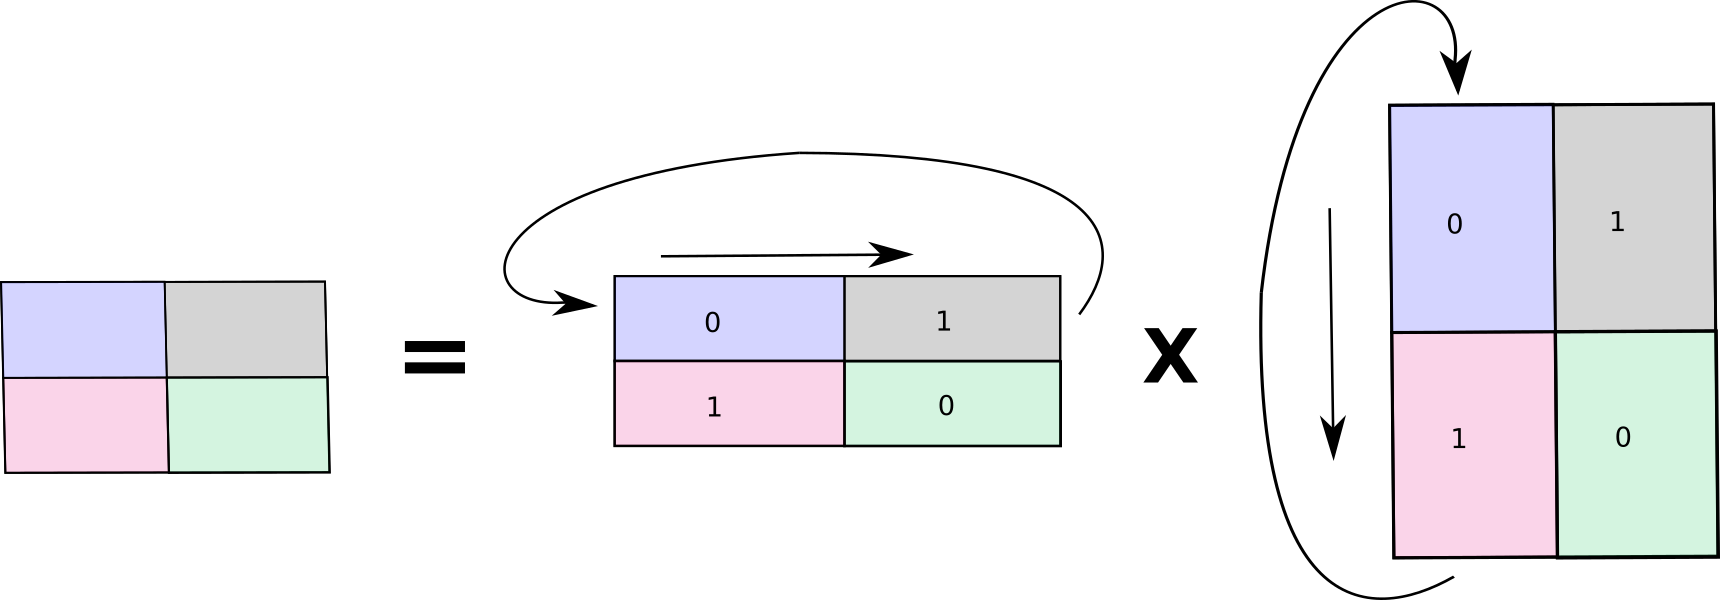
\includegraphics[width=.9\linewidth]{figures/fig_2_2.png}
\end{subfigure}
\begin{subfigure}{.9\textwidth}
  \centering
  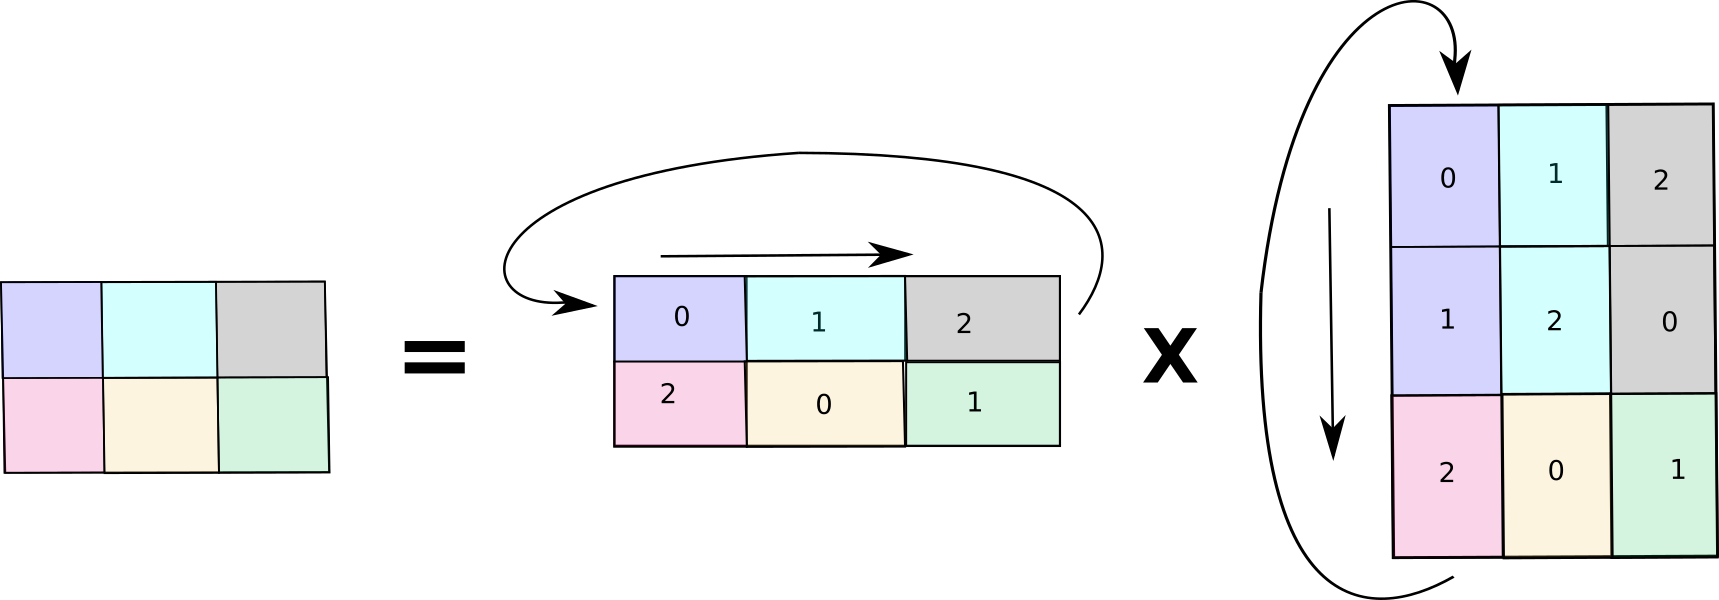
\includegraphics[width=.9\linewidth]{figures/fig_2_3.png}
\end{subfigure}
\caption{Examples of the data decomposition. Each color represents a different process. 
The numbers indicate the initial data placement in terms of which block along the shared dimension
the data is from. For instance, if the numbers in a column in matrix B are 2, 0, 1, the column has 
been rotated once.}
\label{fig:fig}
\end{figure}

I evaluated this algorithm with OpenBLAS as well as the matrix multiplication implementation that I did for 
the last homework. This is so the efficacy of the distributed matrix multiplication algorithm can
be assessed independently from the shared memory matrix multiplication algorithm used. I used only the
non-blocking MPI functions for both send and receive. Both are started before the matrix multiplication
each step, and the wait for completion happens after the multiplication. Additional memory
is required to do this. In the case where there is just one process in the data communication ring,
I still use MPI to communication with itself. This case could be further optimized at the cost of some
simplicity.

\section{}

The roof-line model will be evaluated for square grids of processes for simplicity though the analysis
will generally apply to other cases.
The total number of FLOPs used by this algorithm is the same as the number of FLOPs used in standard
shared memory matrix multiplication. The number of times the data is passed between processes is
$\sqrt{d} - 1$ if $d$ is the number of processes. The total memory bandwidth will be the number
of times data is passed between processes multiplied by the combined size
size of matrices A and B and the memory bandwidth for standard matrix multiplication. This counts memory
bandwidth associated with MPI communication.
If the dimension of A is $n \times n$, the dimension of B is $n \times n$, and the bigger of the two
previous block dimensions is $d$, the total number of FLOPs
used is $2 n^3$ and the total memory that must be transfered in bytes is 
$ 8 * 3 * (\sqrt{d} - 1) * n^2 + 8 * 3 * n^2 = 24 * \sqrt{d} * n^2$. The arithmetic intensity is 
$\frac{2 n^3}{24 * \sqrt{d} * n^2} = \frac{n}{12 * \sqrt{d}}$ The CPUs used in the CCV are Intel Xeon 
model number 6126. According to the Intel specification found 
\href{https://www.intel.com/content/www/us/en/support/articles/000005755/processors.html}{here}: 
the CPU has 652.8 
peak GFLOPS. The peak memory bandwidth should be about 100 gigabytes per second based on the
memory bandwidth of other similar CPUs. As such, the ratio of peak FLOPS to peak memory bandwidth 
is approximately $(\frac{652.8}{100} = 6.528)$. So long as $\frac{n}{12 * (d + 1)}$ is greater
than 6.528, the computation will ideally be FLOP limited. For values of $n$ in the range
2,048 to 16,384 and $d$ between 1 and 64, the computation should be FLOP limited. \\

This previous computation doesn't factor in that MPI message passing will be substantially slower than
the peak memory bandwidth. The total MPI memory bandwidth is $24 * (\sqrt{d} - 1)  * n^2$. I attempted to test the 
between process memory bandwidth, but the bandwidth seems too low (around 4 GB/s). If this 
is assumed to be accurate, then the computation has an effective MPI ratio of peak FLOPS to 
peak memory bandwidth of $(\frac{652.8}{4} = 163.2)$  The effective MPI arithmetic intensity
is $\frac{n}{12 * (\sqrt{d} - 1)}$, so MPI communication will be limiting for some values of $n$ and $d$
within the scope of this computation. For instance, the computation will theoretically be MPI bandwidth
limited for $n = 2048$ and $d = 9$ and $n = 4096$ and $d = 16$.

\section{}

\begin{table}[]
\begin{centering}
\begin{tabular}{|l|l|l|l|}
\hline
Implementation & n    & Seconds   & GLOPS   \\ \hline
Naive          & 512  & 0.0249    & 10.5    \\ \hline
Optimized      & 512  & 0.00427   & 60.0    \\ \hline
Eigen          & 512  & 0.00333   & 75.1    \\ \hline
Naive          & 1024 & 0.181     & 11.0    \\ \hline
Optimized      & 1024 & 0.0335    & 59.6    \\ \hline
Eigen          & 1024 & 0.0127    & 158.1   \\ \hline
Naive          & 2048 & 11.9      & 1.3     \\ \hline
Optimized      & 2048 & 0.338     & 47.4    \\ \hline
Eigen          & 2048 & 0.0805    & 198.7   \\ \hline
\end{tabular}
\caption{Performance with the '-march=native' compiler argument}
\end{centering}
\end{table}


\begin{table}[]
\begin{centering}
\begin{tabular}{|l|l|l|l|}
\hline
Implementation & n    & Seconds   & GLOPS   \\ \hline
Naive          & 512  & 0.0244    & 10.2    \\ \hline
Optimized      & 512  & 0.00797   & 31.4    \\ \hline
Eigen          & 512  & 0.00403   & 62.0    \\ \hline
Naive          & 1024 & 0.221     & 9.04    \\ \hline
Optimized      & 1024 & 0.0642    & 31.1    \\ \hline
Eigen          & 1024 & 0.0199    & 100.6   \\ \hline
Naive          & 2048 & 12.2      & 1.3     \\ \hline
Optimized      & 2048 & 0.675     & 23.7    \\ \hline
Eigen          & 2048 & 0.243     & 65.9    \\ \hline
\end{tabular}
\caption{Performance without '-march=native'}
\end{centering}
\end{table}

\end{document}

